\documentclass[a4paper, 11pt]{article}
\usepackage{pgfgantt}
\usepackage{fancyhdr}
\usepackage{textcomp}
\usepackage{graphicx}



\fancypagestyle{title}{
\renewcommand{\headrulewidth}{0pt}
\fancyhf{}
\lhead{Luke Bessant - 2019}
\rhead{}
}
\pagestyle{title}

\title{\textbf{CS3821 Full Unit Project}\\On Lexical Analysis}
\author{Luke Bessant\\Supervisor: Reuben Rowe}
\date{November 2, 2019}

\begin{document}

\maketitle
\thispagestyle{title}
\newpage

\tableofcontents
\newpage

\section{Introduction}
As the first stage in the compiler toolchain, lexical analysis takes the raw source code of a program written in a language supported by the compiler and processes it in such a way that the program is split up into \textit{lexemes}, which by their character pattern are identified as particular \textit{tokens}, and then passed to the parser for syntax analysis.

\section{The Purpose of Lexical Analysis}
The first step in learning the purpose lexical analysis is understanding \textit{lexemes} and \textit{tokens}. Lexemes are sequences of characters which match the pattern for a particular component of the programming language supported by the compiler. These lexemes represent the individual parts which make up a statement or expression within a program. For example, take the expression below:

\begin{center}
	\texttt{sum = sum + 50}
\end{center}

As humans we can see that this expression is split into the lexemes \texttt{sum}, \texttt{=}, \texttt{sum}, \texttt{+} and \texttt{50}. Thus we are able to tell that this simply adds 50 to the current value of \texttt{sum} and reassigns the result as \texttt{sum}. Since the lexical analyser simply takes the stream of characters from our source program, it has to create lexemes from a sequence of consecutive characters using the production rules outlined wihtin the grammar for the language. The stream of tokens recognised by the lexical analyser is then sent to the next stage, syntax analysi, which may have requested the next token where the parser and lexer are tightly coupled. Another interesting use of the lexical analysis phase is keeping track of the number of newline characters within a program, allowing us to derive the associated line number whenever an error occurs and gives us the ability to show this in an error message.

\section{Tokens}
A token is a pair of the form \textlangle{}\textit{token-name, token-attribute}\textrangle{} denoting the class and contents of a valid lexeme. Many lexemes can match the pattern for a token, therefore we have the option to use an attribute for the token to give the compiler more information about it. This could be a literal value or a pointer to a position in the program's \textit{symbol table}. Upon discovering a pattern matching a valid token, the lexeme is identified by the lexical analyser as an instance of that token. 

For example, the lexeme \texttt{50} in the above expression could be recognised as an \texttt{integer} token and thus the lexer will create the token \textlangle{}\texttt{integer, 50}\textrangle{}. The lexeme \texttt{sum} could match the pattern of an \textit{identifier}, in which case a possible token could take the form \textlangle{}\texttt{id, 1}\textrangle{}. Here \texttt{id} is shorthand for identifier, and \texttt{1} is a pointer to a location within the program's symbol table where more information about the identifier is held, such as the identifier's name, type and current value. Some of the common token types across programming languages are as follows:

\begin{itemize}
\item A token for all identifiers within the language.
\item A token for the keywords within a language, such as \texttt{if} and \texttt{else}.
\item One token all mathematical and boolean operators, or one for each individually.
\item Tokens for literal strings and types of numbers supported by the language.
\item Tokens for punctuation symbols such as brackets, commans and semi-colons.
\item A token for whitespace, which is usually not passed to syntax analysis but is instead omitted by the lexer.
\end{itemize}

\subsection{Attributes of Tokens}
In cases where many lexemes match the pattern of a token, we need to pass more information about the lexeme to the parser so the correct incantation can be properly reproduced in the code generation phase of the toolchain. Therefore the name of the token is used within the parser to make decisions about program structure, whereas the attribute value is used later on when translating tokens during code generation. From the above example, we have \textlangle{}\texttt{integer, 50}\textrangle{}.

For the identifiers of a program we need to encompass several pieces of information within one token, such as the name, type and current value of the identifier. In these cases the token attribute would point to an entry in the program symbol table where this information is held. As we saw from the previous section, an example of this is \textlangle{}\texttt{id, 1}\textrangle{} where \texttt{1} represents row one within the symbol table.

For keywords and operations of which the raw characters of the lexeme match the token name, we can simply omit the attribute and use only the token name within the token. An example of this could be \texttt{if}, where we can discard the attribute value, which matches the token name, and simply use the token \textlangle{}\texttt{if}\textrangle{}.

\subsection{Recognition of Tokens}
We can begin to identify tokens within a program by considering the grammar of the language we are using. All of the clauses within a program should satisfy at least one of the production rules listed within our grammar, otherwise they are invalid. Using finite-state automata we can model each of the production rules by converting their regular expression to a set of states with transitions between them. For instance we have the following finite-state automata for a production \texttt{id} \textbf{\textrightarrow} \texttt{letter(letter|digit)*}:

\begin{figure}[ht!]
	\centering
	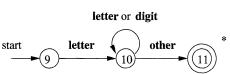
\includegraphics[width=60mm]{/home/luke/Pictures/FA.png}
	\caption{Showing the finite-state automata for \texttt{id} (figure 3.14 from \textit{Aho - Compilers - Principles, Techniques, and Tools - page 132)} \label{overflow}}
\end{figure}

The above example supports the above production rule, allowing only patterns beginning with at least one letter, and then allowing any number of letters or numbers following this. Once we have identified some character which is not a letter or number, we have then reached the end of the identifier name; this is our \textit{accepting} state (denoted by a doubly lined circle). The asterisk atop the accepting state signifies that the last character of the lexeme (\textbf{other}) is not a valid member of the pattern for this token and so the \textit{forward pointer} of the scanner is retracted by one character so as to point to the last character of the identifier. Therefore we can determine that any sequence of characters leading to the accept state of this finite-state automata is an identifier as defined by our grammar.

\newpage
\addcontentsline{toc}{section}{References}
\begin{thebibliography}{9}

\bibitem{Aho} 
Aho, A. Lam, M. Sethi, R. Ullman, J.
[\textit{Compilers - Principles, Techniques, and Tools: Second Edition}]. 
2007.


\end{thebibliography}

\end{document}
